
\chapter{Introduction}


% \section{Contextualization}


    % [IA-GEN NA INDUSTRIA] 
    In the dynamic and ever-changing oil and gas (O\&G) industry,
    \abbrev{O\&G}{Oil and Gas} 
    digital transformation has emerged as a key element to achieve operational efficiency, sustainability, and competitiveness. 
    At the forefront of this transformation are Large Language Models \abbrev{LLM}{Large Language Model}(LLM), which have the potential to process unstructured queries, map out courses of action, and advise users on possible solutions to industrial problems \citep{Kar2023}. 
    We also note the advantage of increased engagement, cooperation, accessibility, and ultimately profitability. 
    These models redefine paradigms in knowledge management and information retrieval and impact a variety of other areas \citep{Eckroth2023}, making it crucial to adopt these technologies to remain competitive.    
    
    % [ESTUDO AUMENTO PRODUTIVIDADE] 
    A study conducted by \citet{Dellacqua2023}, in collaboration with the Boston Consulting Group, shows that in knowledge-intensive tasks, consultants equipped with access to LLMs such as GPT-4 not only completed tasks more efficiently (25.1\% more quickly on average) but also with substantially higher quality, achieving results more than 40\% better compared to those without AI assistance \citep{Dellacqua2023}.
    Increase in productivity of knowledge workers was 12\% on average.    
    A major oil company spent in 2023 \$2.8B with employee compensation \citep{Petrobras2024}.
    A potential increase of 12\% in knowledge workers productivity, given they represent 60\% of all employee, could represent \$204M annual savings in this scenario. 

    
    % [AUMENTO DO PIB DEVIDO A GEN AI] 
    Broader economic indicators predict significant transformations due to generative AI (Gen-AI) across various industries.
    A report from Goldman Sachs \citep{Hatzius2023} highlights that Gen-AI is poised to increase global GDP by nearly 7\%, increasing productivity growth by 1.5 percentage points over the next decade. 
    This economic uplift is expected due to AI's ability to automate complex workflows and create new business opportunities, significantly impacting employment and productivity sectors worldwide.


            
    % [PROBLEMA DE DADOS NA INDUSTRIA EM GERAL] 
    Expanding on the broader discussion on data utilization within organizations, an important issue is the challenge of extracting relevant information from extensive databases \citep{Singh2023}. 
    Initially, the challenge of knowing, finding, and accessing data poses a significant obstacle to decision-making processes. 
    Collaborators at O\&G companies often face the intensive task of manually searching large data repositories to find useful information.


    
    % [PROBLEMA DE DADOS NO O\&G] 
    Focusing specifically on the activities of drilling and completion of offshore and onshore wells, a major challenge lies in the inherently complex and technical nature of the data involved, which can be from various types: operations, projects, technologies, supply chains, and others. 
    Inefficiency in leveraging large volumes of unstructured data increases these challenges, as observed by \citet{Singh2023}. 
    A significant amount of the data generated and collected in this sector is unstructured, ranging from text reports and emails to images and videos of exploration and production activities. 
    Examples include hundreds of daily operational reports from drilling rigs, well execution projects, nonproductive time (NPT)\abbrev{NPT}{Nonproductive Time} reports, and documents of operational lessons learned, as illustrated in Figure \ref{fig:report_example}. 
    As a result, valuable information can remain untapped, and the potential to find insights, informed decision-making, and innovation is significantly compromised.
    \citet{Singh2023} showcases the capabilities and potential of Generative AI-enabled chatbots for the O\&G sector, particularly in enhancing drilling and production analytics to achieve better business results. The author concludes that companies that adopt these technologies in the coming years will see clear advantages.     
    
    \begin{figure}[t]
        \centering
        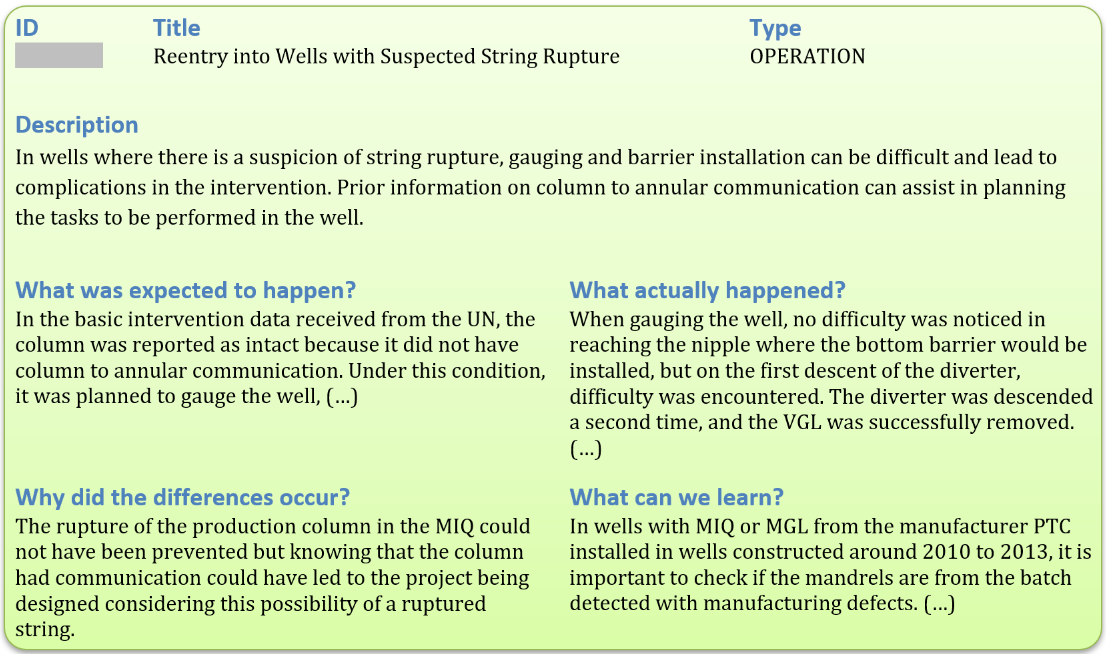
\includegraphics[width=1\textwidth]{images/report_example.png}
        \caption{Sample of drilling \& completion learned lesson partial document. (translated from Portuguese)}
        \label{fig:report_example}
    \end{figure}           
    
    However, the deployment of such technologies presents limitations and introduces challenges, including biased data, hallucinations\footnote{Information that is incorrect or simply fictional.}, lack of explainability, and logical reasoning errors, among others \citep{Hadi2023}, which require a balanced approach to harness their potential in a responsible manner.    
    Although previous research has focused mainly on the broader applications of AI in industry, the novelty of our research lies in its original examination of the specific challenges and solutions presented by the complex, technical and unstructured data inherent in O\&G operations. 
    By comparing single- and multi-agent systems, this study fills a knowledge gap, providing empirical insights into the effectiveness of different Gen-AI architectures in a domain where such studies are scarce. 
    
    The adoption of these technologies by a major oil company underscores their potential to revolutionize data analysis and management, presenting an opportunity for deeper exploration and application.

\section{Business Scope Delimitation}

    To contextualize the scope of this study, it is necessary to understand the life cycle of an oil field, which begins with Exploration and progresses to the Development of Production, followed by effective Production, and culminates in Decommissioning \citep{Badiru2016}. Gen-AI has the potential to impact each of these phases, but the focus of this work lies in the operations of the development and maintenance stages.
            
    Well construction is a highly specialized activity that involves drilling and completion of wells for hydrocarbon extraction \citep{Thomas2004}. In this context, Gen-AI can be applied in various ways. 
    For example, a chatbot could manage knowledge by answering queries about operations and well projects by retrieving information from the organization's databases. 
    Additionally, LLM-based agents could be used in executive project review to ensure that drilling or completion operations comply with the organization's standards and adhere to best operational practices. 
    Moreover, Gen-AI could perform inference in unstructured databases to extract specific information from text reports and obtain structured data. This business scope emphasizes the importance of Gen-AI in the construction and maintenance of wells.

    \subsection{Key Information Sources in Well Engineering} \label{sec:information-sources}

        To fully appreciate the challenges in this domain, it is important to understand the primary data sources that specialists interact with daily. The following sources, used in this research's experiments, exemplify the complex information landscape of well engineering:

        \paragraph{Operational Learned Lessons.} During drilling, completion, and workover interventions, documents called Knowledge Items are written by specialists, as depicted in Fig~\ref{fig:report_example}. These can be of four types: Technical Alert, Learned Lesson, Good Practice, and Well Observation. This system serves as a critical tool for knowledge management, considering the large number and variety of specialists involved and well operations performed.

        \paragraph{Operational NPTs (Non-Productive Time).} This data source contains structured records of anomalies that occurred during well interventions, detailing the title, description, location, operation type, responsible sector, rig involved, time lost, and event dates. These data are critical for the industry, as NPTs represent periods when operations are interrupted. The identification and analysis of these events are essential for continuous process improvement, cost reduction, and increased operational efficiency.

        \paragraph{Collaborator Finder.} The third data source is a collaborator finder, an important internal tool for consulting and managing employee data. This system allows for the quick identification of employees through information such as name, workplace, and role. The importance of this tool lies in the ability to cross-reference employee data with operational events, enabling a more complete analysis by an intelligent agent.

\section{Objectives}

    The primary goal of this dissertation is to systematically evaluate and compare the effectiveness, efficiency, and practical viability of different LLM-based architectures for resolving domain-specific information retrieval challenges in well construction engineering. 
    This research aims to move beyond generalized performance metrics to provide specific, empirical insights into how architectural choices impact outcomes in a industrial setting.

    To achieve this overarching goal, the following specific objectives have been defined:

    \begin{enumerate}
        \item \textbf{Design and Implement LLM Artifacts:} designing and implementing a set of distinct retrieval-augmented generation (RAG)
        \abbrev{RAG}{Retrieval-Augmented Generation} 
        architectures, including non-agentic (baseline and router-based) and agentic (single-agent and multi-agent) systems, tailored to the operational context of well construction.

        \item \textbf{Evaluate Performance Quantitatively:} evaluating the performance of these artifacts on domain-specific tasks using both expert-led qualitative assessments and automated quantitative metrics, including truthfulness, precision, recall, and F1-score.

        \item \textbf{Analyze Cost-Effectiveness:} conducting a comparative analysis of the economic efficiency of each architecture, focusing on the trade-offs between performance gains and the computational costs associated with LLM API usage.

        \item \textbf{Derive Actionable Guidance:} identifying the key challenges, limitations, and failure modes of each architecture within a specialized technical domain, and to derive practical, evidence-based guidelines for the strategic adoption of these technologies in the oil and gas industry.
    \end{enumerate}




\section{Research Questions} \label{sec:research_questions}

    To guide this investigation and structure the research, the study addresses a central research question, which is broken down into three specific sub-questions. These questions will be formally answered in the conclusion, based on the evidence gathered from the two experimental cycles.

    \vspace{\baselineskip}
    \begin{tcolorbox}[colback=gray!10, colframe=gray!40, title=\textbf{Main Research Question}]
    How do different LLM based architectures, ranging from non-agentic RAG pipelines to multi-agent systems, compare in terms of performance, efficiency, and practical viability when applied to domain-specific information retrieval tasks in well construction engineering?
    \end{tcolorbox}
    \vspace{\baselineskip}

    \paragraph{RQ1: Performance and Task-Dependency} Which architecture (non-agentic, single-agent, or multi-agent) provides the highest factual accuracy and overall performance for different types of domain-specific tasks, specifically complex Question-Answering (Q\&A)\abbrev{Q\&A}{Question-Answering} and structured Text-to-SQL generation?

    \paragraph{RQ2: Cost-Effectiveness} What is the relationship between architectural complexity and economic cost? How do the performance benefits of more complex systems (e.g., multi-agent) weigh against their significantly increased computational (API) costs, and what are the implications for practical deployment?

    \paragraph{RQ3: Agentic Systems and Domain Specificity} Under what conditions do agentic architectures, with their capacity for cyclical reasoning and reflection, offer a tangible performance advantage over simpler, non-agentic RAG workflows in a highly specialized technical domain where the LLM has a significant ``knowledge deficit''?

    \vspace{\baselineskip}

    To answer these questions, this research was conducted through two distinct experimental cycles. The first, carried out in 2024, established a foundational comparison, revealing that while a multi-agent architecture achieved 28\% higher truthfulness in Q\&A tasks, its cost was on average 3.7 times higher. Furthermore, a single-agent architecture proved to be surprisingly more effective in Text-to-SQL tasks.

    The rapid evolution of generative AI frameworks and models prompted a second, more advanced experiment in 2025. This second phase built upon the initial findings, employing non-agentic workflows as a baseline and a more rigorous, automated evaluation methodology based on the ``LLM-as-a-Judge'' concept \citep{Gu2025}. This led to a crucial and counter-intuitive discovery: a non-agentic architecture using an intelligent router to select the correct knowledge source decisively outperformed both single and multi-agent systems. This finding suggests that in specialized domains where the LLM lacks deep pre-trained knowledge, the reflective capabilities of agentic systems are less effective than a streamlined, well-directed retrieval process, fundamentally shaping the answers to our research questions.



\section{Research Methodology}
  
    This research follows the Design Science Research (DSR)\abbrev{DSR}{Design Science Research} methodology, a framework particularly suited for studies that develop and evaluate technological artifacts to address specific organizational problems. DSR provides a structured approach for creating innovative solutions while maintaining scientific rigor through empirical validation \citep{hevner2007three}.
    
    \begin{figure}[h]
        \centering
        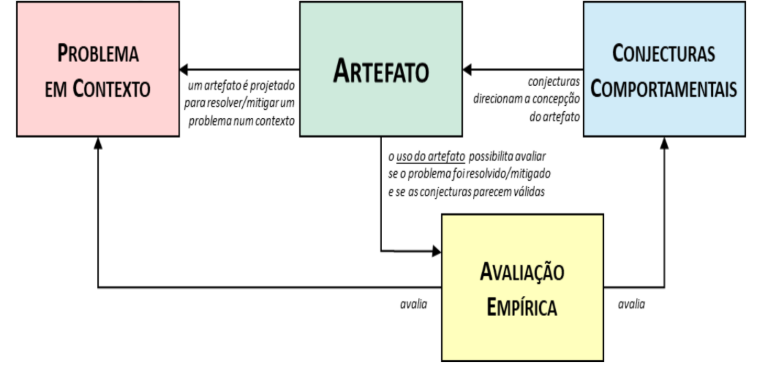
\includegraphics[width=0.8\textwidth]{images/dsr-model.png}
        \caption{Main elements of DSR-Model, translated from \citet{Oswald2023}.}
        \label{fig:dsr-model}
    \end{figure}
    
    \subsection{Design Science Research Framework}
    
        The DSR methodology employed in this study consists of four interconnected elements, as illustrated in Figure~\ref{fig:dsr-model}:
        
        \begin{enumerate}
        \item \textbf{Problem in Context}: Identifying and defining a relevant organizational challenge within its specific environment
        \item \textbf{Artifact}: Designing and developing a technological solution to address the identified problem
        \item \textbf{Behavioral Conjectures}: Formulating hypotheses about how the artifact will function and impact the problem space
        \item \textbf{Empirical Evaluation}: Systematically testing the artifact to validate its effectiveness and the underlying conjectures
        \end{enumerate}
        
        This cyclical framework guides both the research design and execution, ensuring that the developed artifacts are not only technically sound but also practically relevant.
    
    \subsection{Application of DSR in This Research} \label{sec:dsr-application}
        
        \subsubsection{Problem in Context}
        
        This study addresses the challenge of efficiently extracting relevant information from extensive technical databases in the oil and gas industry, specifically in well construction and maintenance operations, as listed in Table~\ref{tab:problem-context}. 
        
        \begin{table}[h]
            \centering
            \caption{Characteristics of the Problem Context}
            \begin{tabular}{|p{0.45\textwidth}|p{0.45\textwidth}|}
            \hline
            \textbf{Challenge Aspect} & \textbf{Description} \\
            \hline
            Data Structure & Large volumes of unstructured data (operational reports, lessons learned documents, NPT reports) \\
            \hline
            Technical Complexity & Domain-specific terminology, complex relationships and tacit knowledge \\
            \hline
            Business Impact & Significant potential economic impact from improved knowledge access \\
            \hline
            \end{tabular}
            \label{tab:problem-context}
        \end{table}
        
        \subsubsection{Artifacts}
        
        Four primary artifacts were designed and implemented across the two experimental cycles, illustrated in Figure~\ref{fig:artifacts}, using state-of-the-art language models and integrated with domain-specific knowledge bases through various retrieval mechanisms.
        
        \begin{figure}[h]
        \centering
        
        \begin{minipage}{0.45\textwidth}
            \centering
            \fbox{\parbox[c][3.8cm][c]{\linewidth}{\centering
                \textbf{Linear-Flow (Baseline)} \\
                \small Non-agentic RAG pipeline with a \\
                \small single sequential LLM step that \\
                \small queries all tools and synthesizes\\
                \small the answer}}
        \end{minipage}
        \hfill
        \begin{minipage}{0.45\textwidth}
            \centering
            \fbox{\parbox[c][3.8cm][c]{\linewidth}{\centering
                \textbf{Linear-Flow with Router} \\
                \small Non-agentic pipeline with an initial \\
                \small routing LLM call that selects the most \\
                \small appropriate tool(s) before retrieval}}
        \end{minipage}
        \vspace{0.6em}
        
        \begin{minipage}{0.45\textwidth}
            \centering
            \fbox{\parbox[c][3.8cm][c]{\linewidth}{\centering
            \textbf{Single-Agent LLM System} \\
            \small A centralized architecture where one \\
            \small language model agent handles the entire \\
            \small question-answering process with \\
            \small access to multiple tools}}
        \end{minipage}
        \hfill
        \begin{minipage}{0.45\textwidth}
            \centering
            \fbox{\parbox[c][3.8cm][c]{\linewidth}{\centering
            \textbf{Multi-Agent LLM System} \\
            \small A collaborative architecture where \\
            \small multiple specialized agents work together \\
            \small under coordination to process queries}}
        \end{minipage}
        \caption{Primary artifacts developed and evaluated across the two experimental cycles.}
        \label{fig:artifacts}
        \end{figure}
        
        
        \subsubsection{Behavioral Conjectures}
        
        The research was guided by several key conjectures:
        
        \begin{tcolorbox}[colback=gray!10, colframe=gray!40, title=Key Research Conjectures]
            \begin{itemize}
            \item Multi-agent systems will demonstrate higher accuracy in complex technical queries due to their ability to distribute cognitive load and specialize in different aspects of the problem
            \item The performance advantages of multi-agent systems will vary by task type (Q\&A vs. Text-to-SQL)
            \item More advanced language models will yield better performance but at significantly higher LLM financial costs
            \item The economic efficiency (performance-to-cost ratio) will be a critical factor in determining practical implementation viability
            \end{itemize}
        \end{tcolorbox}
        
        \subsubsection{Empirical Evaluation}
        
        The evaluation was conducted through two distinct experimental phases (summarized in Table~\ref{tab:experiments}), allowing for iterative refinement of both the artifacts and the evaluation methodology, addressing limitations identified in the first experiment while adapting to the rapid evolution of language model capabilities.
        
        \begin{table}[h]
        \centering
        \caption{Comparison of Experimental Phases}
        \begin{tabular}{|p{0.15\textwidth}|p{0.38\textwidth}|p{0.38\textwidth}|}
        \hline
        \textbf{Aspect} & \textbf{First Experiment (2024)} & \textbf{Second Experiment (2025)} \\
        \hline
        Focus & Comparative analysis of single and multi-agent architectures & Extended evaluation incorporating non-agentic workflows as baseline \\
        \hline
        Evaluation Methods & Expert validation by domain specialists & Automated assessment using LLM-as-a-Judge approach \\
        \hline
        Metrics & Truthfulness, performance, and LLM cost & Precision, recall, and F1-score \\
        \hline
        Outcomes & Identification of key challenges and limitations & More rigorous quantitative evaluation methodology \\
        \hline
        \end{tabular}
        \label{tab:experiments}
        \end{table}

    

\section{Thesis Structure}


    This dissertation is organized into five main chapters, followed by appendices, to present the research in a logical and structured manner.

    \begin{itemize}
        \item \textbf{Chapter 1 - Introduction:} This chapter introduces the research context within the oil and gas industry, highlighting the challenges of knowledge management in well construction. It defines the business scope, establishes the research objectives and guiding research questions, and outlines the DSR methodology that structures the study.

        \item \textbf{Chapter 2 - Literature Review:} This chapter provides the theoretical foundation for the research. It reviews the key concepts of LLMs, RAG, and the architecture of both single and multi-agent systems. It also covers the evaluation methodologies pertinent to this work, including traditional metrics and the LLM-as-a-Judge paradigm.

        \item \textbf{Chapter 3 - First Experimental Evaluation Cycle:} This chapter details the initial experiment comparing single-agent and multi-agent architectures. It follows the DSR framework to describe the artifact design, the expert-led evaluation process, and the results based on metrics of truthfulness, performance, and cost. The findings from this cycle reveal the initial trade-offs and limitations that motivate the second experiment.

        \item \textbf{Chapter 4 - Second Experimental Evaluation Cycle:} This chapter presents a more rigorous and extensive evaluation. It introduces non-agentic workflows as baselines and employs an automated, quantitative evaluation methodology using an LLM-as-a-Judge approach. The results from this cycle provide crucial insights into the performance of different architectures, leading to the central hypothesis of the ``domain knowledge deficit''.

        \item \textbf{Chapter 5 - Conclusion:} This final chapter synthesizes the findings of the entire study. It provides direct answers to the research questions, summarizes the main contributions to theory and practice, acknowledges the limitations of the work, and proposes promising directions for future research.
    \end{itemize}

    Finally, the \textbf{Appendices} provide supplementary material, including the detailed dataset used in the experiments and the source code for the evaluation prompts, to ensure transparency and facilitate reproducibility.
